\setlength{\columnsep}{3pt}
\begin{flushleft}
	\bigskip
	\begin{itemize}
		\item \textbf{One dimensional array}:\par
		
		Once we create an array, every array element is by default initialized with default values.
		
		\begin{figure}[h!]
			\centering
			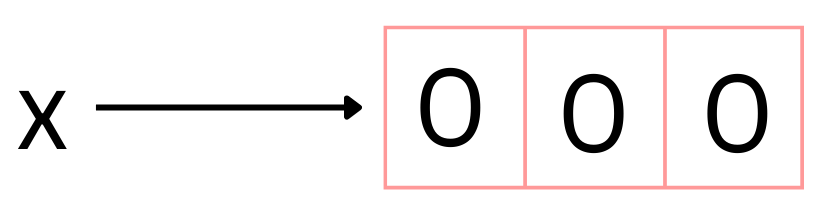
\includegraphics[scale=.45]{content/chapter4/images/new1.png}
		\end{figure}	
		
		
		\begin{tcolorbox}[breakable,notitle,boxrule=1pt,colback=code,colframe=code]
			\color{black}
			\fontdimen2\font=8pt
			int[] a = new int[3]; \par
			System.out.println(a); \par
			System.out.println(a[0]);
			\fontdimen2\font=4pt
		\end{tcolorbox}
		
		Output:
		\begin{tcolorbox}[breakable,notitle,boxrule=-0pt,colback=output,colframe=output]
			\color{black}
			\fontdimen2\font=8pt
			[I@422a8473 \par
			0
			\fontdimen2\font=4pt
		\end{tcolorbox}	
		
		Whenever we are trying to print any reference variable, internally two string method will be called, which is implemented by default to return the string in the following form:
		\par
		\textbf{class\_name@hexadecimal\_form}
		
		\bigskip
		\item \textbf{Two-dimensional array}:  \par
		
		Example 1:
		\begin{figure}[h!]
			\centering
			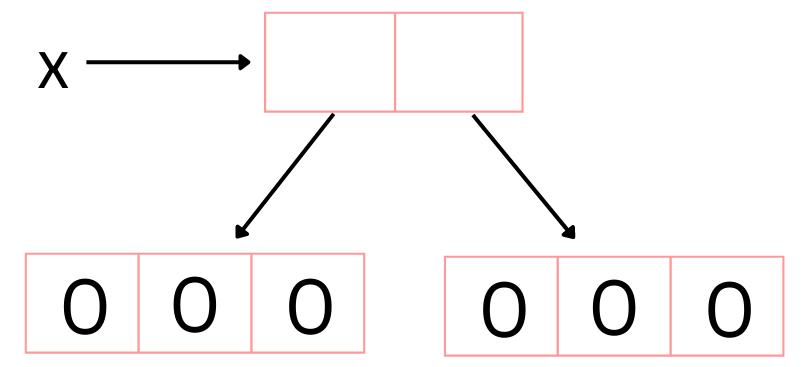
\includegraphics[scale=.45]{content/chapter4/images/new2.png}
		\end{figure}	
		
		\begin{tcolorbox}[breakable,notitle,boxrule=1pt,colback=code,colframe=code]
			\color{black}
			\fontdimen2\font=8pt
			int[][] a = new int[2][3]; \par
			System.out.println(a);  \par
			System.out.println(a[0]);  \par
			System.out.println(a[0][0]);			
			\fontdimen2\font=4pt
		\end{tcolorbox}
		
		Output:
		\begin{tcolorbox}[breakable,notitle,boxrule=-0pt,colback=output,colframe=output]
			\color{black}
			\fontdimen2\font=8pt
			[[I@5a39699c \par
			[I@129a8472  \par
			0
			\fontdimen2\font=4pt
		\end{tcolorbox}	
		
		Example 2:
		
		\begin{figure}[h!]
			\centering
			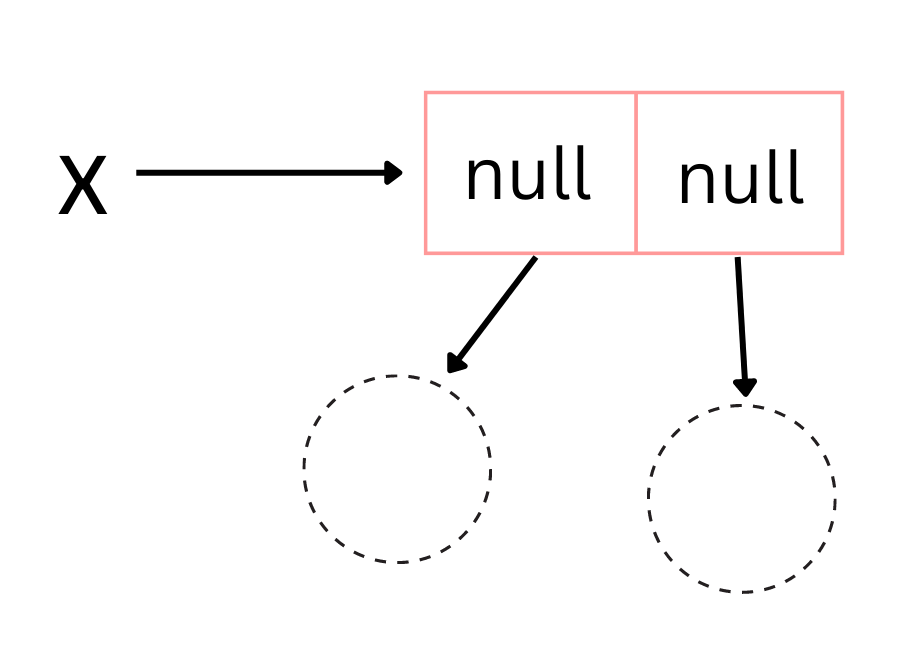
\includegraphics[scale=.45]{content/chapter4/images/new3.png}
		\end{figure}	
		
		\begin{tcolorbox}[breakable,notitle,boxrule=1pt,colback=code,colframe=code]
			\color{black}
			\fontdimen2\font=8pt
			int[][] a = new int[2][]; \par
			System.out.println(a);  \par
			System.out.println(a[0]);  \par
			System.out.println(a[0][0]);			
			\fontdimen2\font=4pt
		\end{tcolorbox}
		
		Output:
		\begin{tcolorbox}[breakable,notitle,boxrule=-0pt,colback=output,colframe=output]
			\color{black}
			\fontdimen2\font=8pt
			[[I@5a39699c \par
			null  \par
			Exception in thread "main" java.lang.NullPointerException: 
			\fontdimen2\font=4pt
		\end{tcolorbox}	
		
		\bigskip
		
		\item \textbf{Over-riding array value:} \par
		Once we create an array, every array element by default initialised with default values. \par
		We can over-ride default values with custom values.
		
		\begin{figure}[h!]
			\centering
			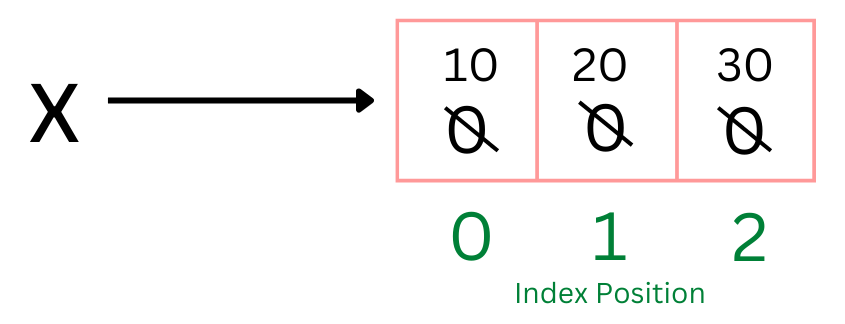
\includegraphics[scale=.45]{content/chapter4/images/image2.png}
		\end{figure}	
		
		\begin{tcolorbox}[breakable,notitle,boxrule=1pt,colback=code,colframe=code]
			\color{black}
			\fontdimen2\font=8pt
			int[] a = new int[3]; \par
			a[0]=10; \par
			a[1]=20; \par
			a[2]=30; \par
			System.out.println(a[0]); \par
			System.out.println(a[1]); \par
			System.out.println(a[2]);
			\fontdimen2\font=4pt
		\end{tcolorbox}
		
		Output:
		\begin{tcolorbox}[breakable,notitle,boxrule=-0pt,colback=output,colframe=output]
			\color{black}
			\fontdimen2\font=8pt
			10 \par
			20 \par
			30 
			\fontdimen2\font=4pt
		\end{tcolorbox}	
		
		Note: Trying to access array element with out of range index (either positive or negative integer value) will result in runtime exception:  \textbf{"ArrayINdexOutOfBoundException"}
		
	\end{itemize}
	
	
\end{flushleft}
\newpage

